\documentclass[%
reprint,
superscriptaddress,
%groupedaddress,
%unsortedaddress,
%runinaddress,
%frontmatterverbose,
%preprint,
showpacs,preprintnumbers,
%nofootinbib,
%nobibnotes,
%bibnotes,
 amsmath,amssymb,
 aps,
%pra,
%prb,
prd,
%prl,
%rmp,
%prstab,
%prstper,
%floatfix,
]{revtex4-1}

\usepackage{float}
\usepackage{graphicx}% Include figure files
\usepackage{dcolumn}% Align table columns on decimal point
\usepackage{bm}% bold math
\usepackage{bbold}
\usepackage{amssymb,amsmath}
\usepackage{hyperref}% add hypertext capabilities
%\usepackage[mathlines]{lineno}% Enable numbering of text and display math
%\linenumbers\relax % Commence numbering lines

%\usepackage[showframe,%Uncomment any one of the following lines to test
%%scale=0.7, marginratio={1:1, 2:3}, ignoreall,% default settings
%%text={7in,10in},centering,
%%margin=1.5in,
%%total={6.5in,8.75in}, top=1.2in, left=0.9in, includefoot,
%%height=10in,a5paper,hmargin={3cm,0.8in},
%]{geometry}



\usepackage{color}
\usepackage{amsfonts}
\usepackage{subfigure}
\usepackage{array}


\newcommand{\Tr}{\ensuremath{\operatorname{Tr}}}
\newcommand{\tr}{\ensuremath{\operatorname{tr}}}
\newcommand{\Omegaqq}{\ensuremath{\Omega_{\bar{q}q}}}
\newcommand{\vev}[1]{\ensuremath{\left\langle #1 \right\rangle}}
\newcommand{\einh}[1]{\ensuremath{\,\text{#1}}}
\newcolumntype{L}{>{\centering\arraybackslash}m{3cm}}



\newcommand{\overbar}[1]{\mkern 1.5mu\overline{\mkern-1.5mu#1\mkern-1.5mu}\mkern 1.5mu}

\definecolor{bjcol}{rgb}{1,.44,0.13}

% color def's

\definecolor{blue}{rgb}{0,0,1}
\newcommand{\colb}[1]{{\color{blue} #1}}
\definecolor{green}{rgb}{0,1,0}
\newcommand{\colg}[1]{{\color{green} #1}}
\definecolor{red}{rgb}{1,0,0}
\newcommand{\colr}[1]{{\color{red} #1}}
\newcommand{\colJ}[1]{{\color{cyan} #1}}
\definecolor{gray}{rgb}{.5,.5,.5}
\newcommand{\drop}[1]{{\sout{ {\color{gray} #1}}}}
\definecolor{darkgreen}{rgb}{.0,.5,.0}
\newcommand{\colL}[1]{{\color{darkgreen} #1}}


\def\Fig#1{Fig.~\ref{#1}} \def\Tab#1{Tab.~\ref{#1}}
\def\Figs#1{Figs.~\ref{#1}} \def\Tab#1{Tab.~\ref{#1}}
\def\Eqs#1{Eqs.~(\ref{#1})}
\def\Eq#1{Eq.~(\ref{#1})}
\def\eq#1{(\ref{#1})}
\def\eqref#1{(\ref{#1})}
\def\fig#1{Fig.~\ref{#1}}
\def\tab#1{Tab.~\ref{#1}}
\def\eqs#1{(\ref{#1})}
\def\Eqs#1{(\ref{#1})}
\def\sec#1{Sec.~\ref{#1}}
\def\app#1{Appendix~\ref{#1}}
\newcommand{\Phibar}{\ensuremath{\bar{\Phi}}}
\newcommand{\LPQM}{\ensuremath{\mathcal{L}_{\textrm{PQM}}}\xspace}

\def\dbar{{\mathchar'26\mkern-12mu d}}
\def\lA0{{\langle A_0 \rangle}}
\def\bA0{{\bar{A}_0}}
\def\lLA{{\langle L[A_0] \rangle}}
\def\lL{{\langle L \rangle}}
\def\lLc{{\langle L^\dagger \rangle}}
\def\lLAc{{\langle L^\dagger[A_0] \rangle}}


\def\dr{{D\!\llap{/}}\,}
\def\Dr{{D\!\llap{/}}\,}
\def\ipv{\vec{p}\llap{/}}
\def\pslash{p\llap{/}}

\def\0#1#2{\frac{#1}{#2}}

\newcommand{\bsig}{\ensuremath{\bar{\sigma}}}
\newcommand{\lsm}{L\ensuremath{\sigma}M\xspace}
\newcommand{\pT}{\ensuremath{T_0}}
\newcommand{\Tl}{\ensuremath{T_\chi}}
\newcommand{\Ts}{\ensuremath{T_\chi^s}}
\newcommand{\Tchi}{\ensuremath{T_\chi}}
\newcommand{\Td}{\ensuremath{T_d}}
\newcommand{\Tc}{\ensuremath{T_c}}
\newcommand{\muc}{\ensuremath{\mu_c}}
\newcommand{\coloronl}{(color online)\xspace}

\newcommand{\mrm}[1]{\mathrm{#1}}
\def\qbar{\bar{q}}
\newcommand{\sx}{\sigma_{x}}
\newcommand{\sy}{\sigma_{y}}

%%%%%%%%%%%%%% for corrections %%%%%%%%%%%
\newcommand{\colsy}[1]{\textcolor{blue}{#1}}
\newcommand{\colrw}[1]{\textcolor{cyan}{#1}}
\newcommand{\colwjf}[1]{\textcolor{red}{#1}}

%
%%%%%%%%%%%%%%%%%%%%%%%%%%%%%%%%%%%%%%%%%%%%%%%%%%%%%%%%%%%%%%%%%%%%%%%%%%%%%

\graphicspath{{./figures/}{./}}

\begin{document}

\preprint{}

\title{Mesonic dynamics and QCD phase transition
}

\author{Shi Yin}
\affiliation{School of Physics, Dalian University of Technology, Dalian, 116024,
  P.R. China}

\author{Rui Wen}
\affiliation{School of Physics, Dalian University of Technology, Dalian, 116024,
  P.R. China}

\author{Wei-jie Fu}
\email{wjfu@dlut.edu.cn}
\affiliation{School of Physics, Dalian University of Technology, Dalian, 116024,
  P.R. China}

%\date{\today}% It is always \today, today,
             %  but any date may be explicitly specified

\begin{abstract}
We study the finite temperature and density two flavor quark-meson model under the functional renormalisation group. The effect of broken $O(4)-$ symmetry of the wave function  renormalisation and expansion point of effective potential on the thermodynamic quantities and baryon number fluctuation are investigate. At the same time, the field dependent Yukawa coupling is also considered. We give results of the pion mass, the quark mass, the trace anomaly, the baryon number fluctuation and the freeze-out curve.
\end{abstract}

%\pacs{Valid PACS appear here}% PACS, the Physics and Astronomy
%\pacs{11.30.Rd, %Chiral symmetries
%         11.10.Wx, %Finite-temperature field theory
%        05.10.Cc, %Renormalization group methods
%         12.38.Mh  %Quark-gluon plasma
%     }                             % Classification Scheme.
%\keywords{Suggested keywords}%Use showkeys class option if keyword
                              %display desired
\maketitle

%\tableofcontents

%%%%%%%%%%%%%%%%%%%%%%%%%%%%%%%%%%%%%%%%%%%%%%%%%%%%%%%%%%%
%%%%%%%%%%%%%%%%%%%%%%%%%%%%%%%%%%%%%%%%%%%%%%%%%%%%%%%%%%%

\section{Introduction}
\label{sec:int}


The QCD phase structure and the search of the critical end point (CEP) are the most popular research direction in both experimental and theoretical field. The phase transition between the quark gluon plasma (QGP) and hadron is the main research objects. The research of the QGP-hadron phase transition can help us to help us better understand the nature of elementary particles. The experiment to looking for the QGP is being made at the Large Hadron Collider (LHC) and the Relativistic Heavy-Ion Collider (RHIC).

In terms of theoretical research, there many different methods to investigate the QCD phase structure. The most widely studied method is the lattice QCD. A lot of properties of the QCD matter have been discussed under the lattice simulations. Although the lattice theory has the sign problem at high baryon chemical potential, it still gave us plenty of great outcomes. In order to avoid the problem that occurs in lattice calculation, the study of the continuous non-perturbative field theory is in progress at the same time. For example, the Dyson-Schwinger equation. And the Functional Renormalization Group (FRG) is the other good functional approach of the continuous theory. In these ways we can study the behavior of the strong interaction matter under the finite temperature and density better.

This work is done with the low energy effective model under the FRG approach. 
%%%%%%%%%%%%%%%%%%%%%%%%%%%%%%%%%%%%



The low-energy effective models, e.g. the quark-meson (QM) model \cite{Schaefer:2004en}, Nambu--Jona-Lasinio (NJL) model, and their Polyakov-loop improved variants: PQM and PNJL, are suitable to be employed to study the QCD phase transitions. They have been investigated quite a lot in literatures, see, e.g., \cite{} for more details. In this work, we adopt the scale-dependent effective action for the two-flavor PQM model, as follows 
\begin{align}
\Gamma_k=&\int_x \bigg\{Z_{q,k}\bar{q} \Big [\gamma_\mu \partial_\mu -\gamma_0(\mu+igA_0) \Big ]q \nonumber\\[2ex]
&+\frac{1}{2}\Big [Z_{\phi,k}^{\parallel}(\partial_0 \phi)^2+Z_{\phi,k}^{\perp}(\partial_i \phi)^2 \Big]\nonumber\\[2ex]
&+h_k(\rho)\bar{q}\big(T^0\sigma+i\gamma_5\vec{T}\cdot \vec{\pi}\big)q+V_k(\rho)-c\sigma \bigg\}\,,\label{eq:action}
\end{align}
with $\mu=(0, 1, ..., 3)$ and $i=(1, 2, 3)$. In \Eq{eq:action} we have used notation $\int_{x}=\int_0^{1/T}d x_0 \int d^3 x$, where the imaginary time formalism for the field theory at finite temperature is used, and the temporal length reads $\beta=1/T$. Apparently, when the temperature is nonzero, the $O(4)$-symmetry in the Euclidean space is broken into that of $\mathbb{Z}_2\otimes O(3)$, which leads to the split of the magnetic and electric components of correlations functions. They correspond to the components transversal and longitudinal to the heat bath, respectively. In this work, we take this split into account in the two-point correlation function for the mesons, as shown in the second line on the r.h.s. of \Eq{eq:action}, where $Z_{\phi,k}^{\parallel}$ and $Z_{\phi,k}^{\perp}$ indicate the longitudinal and transversal wave function renormalizations for the temporal and spacial components, respectively. 

The reason why we concentrate on the split of the wave function renormalization especially for the mesons is due to the facts as follows. Firstly, in comparison to the quark wave function renormalization $Z_{q,k}$ and the scale dependent Yukawa coupling $h_k$ in \Eq{eq:action}, it is found that the meson wave function renormalization $Z_{\phi,k}$ plays the most significant role beyond the local potential approximation (LPA) \cite{Pawlowski:2014zaa,Fu:2015naa}. In the LPA, the propagators are classical, i.e., $Z_{q,k}=Z_{\phi,k}=1$ and the Yukawa coupling $h$ is a constant and independent of the scale $k$. Secondly, In Ref. \cite{Helmboldt:2014iya} calculations based on the full momentum-dependent two-point correlation functions of mesons are compared with those from LPA and LPA$'$, and here in LPA$'$ a momentum-independent $Z_{\phi,k}$ is included, and it is found that there is a good agreement between the full momentum calculation and the LPA$'$, while not LPA, which indicates that the dispersion relation for the meson, resulting from a scale dependent $Z_{\phi,k}$, have already captured most momentum dependence of the two-point correlation function. 

Considering the importance of the wave function renormalization for the mesons and the success of LPA$'$, in this work we would like to investigate the effects of the splitting of $Z_{\phi,k}$ in the LPA$'$ as shown in \Eq{eq:action}, which is a natural choice at finite temperature as discussed above. Furthermore, we will also study the interplay between the splitting of $Z_{\phi,k}$ and other truncation approaches, e.g., the field dependent Yukawa coupling $h_k(\rho)$ which encodes higher order quark-meson scattering processes \cite{Pawlowski:2014zaa}, fixed point expansion for the effective potential $V_k(\rho)$ in \Eq{eq:action} versus the physical point expansion, etc. Their influences on the QCD phase transition and observables, e.g. fluctuations of the baryon number, will be investigated in detail.


%%%%%%%%%%%%%%%%%%%%%%%%%%%%%%%%%%%%

\section{Functional renormalization group and flow equations}
\label{sec:FRG}

To proceed, we describe other notations in the effective action in \Eq{eq:action}. $\phi=\left(\sigma,\vec{\pi}\right)$ is a meson field with four components. The effective potential $V_k(\rho)$ with $\rho=\phi^2/2$ is $O(4)$ invariant and the c-term $c\sigma$ breaks the chiral symmetry explicitly. The mesons interact with quarks through the scalar and pseudo-scalar channels with a mesonic field dependent Yukawa coupling $h_k(\rho)$, and $T^0$ and $T^i$ are the generators in the flavor space with the convention as follows: $\Tr(T^{i}T^{j})=\frac{1}{2}\delta^{ij}$ and $T^{0}=\frac{1}{\sqrt{2N_{f}}}\mathbb{1}_{N_{f}\times N_{f}}$ with $N_{f}=2$. Besides the wave function renormalization for the meson, we also introduce one for the quark, i.e., $Z_{q,k}$. Since it plays a minor role in the chiral dynamics in comparison to $Z_{\phi,k}$, the splitting of $Z_{q,k}$ into the transversal and longitudinal components are neglected for simplicity in calculations. Finally, $\mu$ in the first line on the r.h.s. of \Eq{eq:action} denotes the quark chemical potential, and here the temporal gluon background field $A_0$, which encodes the Polyakov dynamics, are also taken into account.

The renormalization group (RG) scale $k$ in \Eq{eq:action} is an infrared cutoff, below which quantum fluctuations are suppressed in the effective action. The evolution of the effective action with $k$ is described by the Wetterich equation \cite{Wetterich:1992yh}, which reads 
\begin{align}
  \partial_t\Gamma_k[\Phi]&=\frac{1}{2}\mathrm{Tr}\big(G_{\phi\phi,k}\partial_t R^{\phi}_{k}\big)-\mathrm{Tr}\big(G_{q\bar{q},k}\partial_t R^{q}_{k}\big)\,, \label{eq:WetterichEqPQM}
\end{align}
with the RG time $t=\ln (k/\Lambda)$ and the initial ultraviolet (UV) cutoff $\Lambda$, where $R^{\phi}_{k}$ and $R^{q}_{k}$ are the regulators for the meson and quark fields, respectively, and they are given in Eqs.~(\ref{eq:Rphi}) and ~(\ref{eq:Rq}). The scale dependent meson and quark propagators are given by
\begin{align}
  G_{\phi\phi/q\bar{q}}[\Phi]=\left( \frac{1}{\frac{\delta^2\Gamma_k[\Phi]}{\delta\Phi^2}+R^{\Phi}_{k}} \right)_{\phi\phi/q\bar{q}}\,, \label{eq:props}
\end{align}
with $\Phi=(q,\bar q,\phi)$ denoting all species of fields.

Inserting the effective action in \Eq{eq:action} into the flow equation \eq{eq:WetterichEqPQM}, one arrives at the flow equation for the effective potential, which reads
\begin{align}
  \partial_t V_k(\rho)=&\frac{k^4}{4\pi^2} \bigg [\big(N^2_f-1\big) l^{(B)}_{0}(\bar{m}^{2}_{\pi,k},\eta^{\perp}_{\phi,k},z_\phi;T)\nonumber\\[2ex]
&+l^{(B)}_{0}(\bar{m}^{2}_{\sigma,k},\eta^{\perp}_{\phi,k},z_\phi;T)\nonumber\\[2ex]
&-4N_cN_fl^{(F)}_{0}(\bar{m}^{2}_{q,k},\eta_{q,k};T,\mu)\bigg]\,,
\end{align}
with the RG invariant dimensionless meson and quark masses as follows
\begin{align}
  \bar{m}^{2}_{\pi,k}&=\frac{V'_k(\rho)}{k^2Z^{\perp}_{\phi,k}}\,, \qquad \bar{m}^{2}_{\sigma,k}=\frac{V'_k(\rho)+2\rho V''_k(\rho)}{k^2 Z^{\perp}_{\phi,k}}\,,\\[2ex]
  \bar{m}^{2}_{q,k}&=\frac{h^{2}_{k}\rho}{2k^2Z^{2}_{q,k}}\,.
\end{align}
The anomalous dimensions for the mesons and quark are given by
\begin{align}
  \eta_{\phi,k}^{\perp}&=-\frac{\partial_t Z_{\phi,k}^{\perp}}{Z_{\phi,k}^{\perp}}\,,\quad \eta_{\phi,k}^{\parallel}=-\frac{\partial_t Z_{\phi,k}^{\parallel}}
{Z_{\phi,k}^{\parallel}}\,,\quad \eta_{q,k}=-\frac{\partial_t Z_{q,k}}{Z_{q,k}}\,, \label{}
\end{align}



\colwjf{I am here}
















\section{Dispersion relationship in the PQM model}
\label{sec:}

The Low-energy effective model is a effective research tool to study the QCD matter under the finite temperature and density. In the 
finite temperature quantum field theory, the $O(4)$-symmetry in the vacuum is broken. The time component of momentum changes into the 
summation of Masubara frequency. The $O(4)$-symmetry changes into a 
$\mathbb{Z}_2\otimes O(3)$ symmetry, which leads to the split of the magnetic component and electric component. These two 
components are related to the transversal and longitudinal direction to the heat bath. This division makes the 4-dimension momentum
into two parts, the Matsubara mode part and the space part. For example, the internal momentum under the finite temperature should 
be divided into $q_0=2\pi T(n+\frac{1}{2})$ and $\vec{q}$. Naturally, this division will divide the propagator into these two parts and 
the wave function renormalization coefficient is also. So we should study the QCD matter in the case of considering the difference 
between the two components of the dressing function $Z$. \par

However, in the past research of the Polyakov-Quark-Meson model under functional renormalization group, we always employ an 
approximation that assume $Z^{\bot}=Z^{\|}$. Under this approximation we can simplify calculations as much as possible without 
losing too much information. Nevertheless, the transversal component plays a major role in the physics we should also study their 
nontrivial influence on the Matsubara frequency and the space momentum.\par

In the theory of the PQM we have two kind of dressing functions, the meson $Z_{\phi}$ and the quark $Z_{q}$. In the previous 
research of PQM model, the approximation that $Z^{\bot}=Z^{\|}=Z$ is widely used. The transversal and longitudinal components are
assumed to be equal. However, the magnitude of this approximation has not been studied. Thus, it is necessary to check the 
reliability of this approximation.\par

In this work, we investigate the affect of the meson dressing function and compare the numerical results which are obtained under 
$Z^{\bot}_{\phi}=Z^{\|}_{\phi}=Z_{\phi}$ with $Z^{\bot}_{\phi}\neq Z^{\|}_{\phi}$. The wave function renormalizations are scale-
dependent, if we want to discuss the affect of them, the numerical calculation must be performed beyond the local potential 
approximation (LPA). The flow of the dressing function should meet the function written below
\begin{align}
\partial_tZ^{\bot}_{\phi,k}\neq 0,\qquad \partial_tZ^{\|}_{\phi,k}\neq 0
\end{align}
Therefore, the flow of $Z_{\phi,k}$ also working in the meson anomalous dimensions, which follows
\begin{align}
\eta_{\phi,k}=-\frac{\partial_tZ_{\phi,k}}{Z_{\phi,k}}\label{eq:anodim1}
\end{align}
With the broken of the $O(4)$-symmetry the meson anomalous dimension will split into

\begin{align}
\eta_{\phi,k}^\bot=-\frac{\partial_tZ_{\phi,k}^\bot}{Z_{\phi,k}^\bot} ,\qquad \eta_{\phi,k}^\|=-\frac{\partial_tZ_{\phi,k}^\|}
{Z_{\phi,k}^\|}\label{eq:anodim}
\end{align}


\begin{figure*}[t]
\label{fig:m}
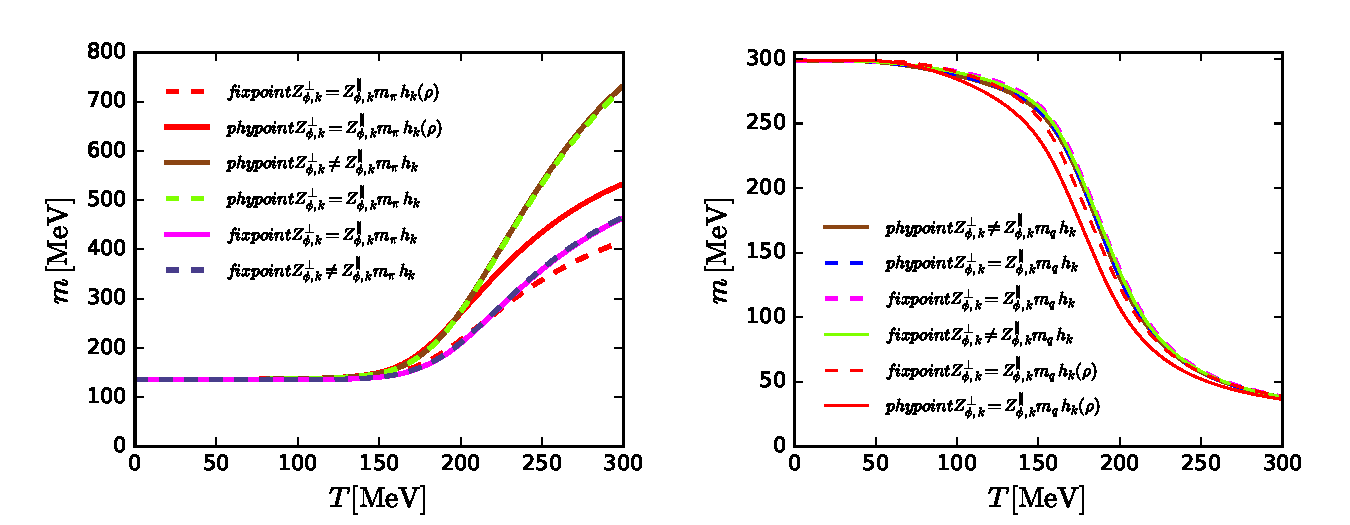
\includegraphics[width=1.0\textwidth]{m.pdf}
\caption{The left diagram is the mass of the pion as a function of temperature, the right curves are the constituent quark mass. 
These diagrams are obtained under fix point and physical point expansion of the effective potential.}
\end{figure*}


%%%%%%%%%%%%%%%%%%%%%%%%%%%%%%%%%%%%%%%%%%%%%%%%%%%



\section{polyakov-quark-meson model under the FRG approximation}
As is shown in the previous work, the Polyakov-quark-meson model of two-flavor can be studied with the flow equation of the 
scale-dependent effective action 
$\Gamma_k[\Phi]$, $\Phi$ is the superfield, it can be written as
 $\Phi=(q,\overline{q},\phi,...)$.  The flow equation within the framework of FRG can be written as
\begin{align}\label{fqm}
\begin{split}
\partial_t\Gamma_k[\Phi]=\frac{1}{2}Tr\big(G_{\phi\phi}\partial_tR^{\phi}_{k}\big)-Tr\big(G_{q\bar{q}}\partial_tR^{q}_{k}\big)
\end{split}
\end{align}
\begin{align}\label{cqm}
\begin{split}
G_{\phi\phi/q\bar{q}}[\Phi]=\left( \frac{1}{\frac{\delta^2\Gamma_k[\Phi]}{\delta\Phi^2}+R^{\Phi}_{k}} \right)_{\phi\phi/
q\bar{q}}
\end{split}
\end{align}

is the propagator which is full field-dependent.
The effective action that depends on the scale of the quark-meson model can be written like this
\begin{align}
\begin{split}
\Gamma_k=\int_x\big\{Z_{q,k}\overline{q} [\gamma_\mu \partial_\mu -\gamma_0(\mu+igA_0) ]q+\frac{1}{2}Z_{\phi,k}
(\partial_\mu \phi)^2\\+h_k\overline{q}
(T^0\sigma+i\gamma_5\vec{T}\cdot \vec{\pi})q+V_k(\rho)-c\sigma \big\}+\cdot\cdot\cdot\label{eq:effact}
\end{split}
\end{align}
here we omited the higher-order terms. The integral sign can be written as $\int_x=\int_0^{1/T}dx_0\int d^3x$.The meson 
field is $\phi=\left(\sigma,\vec{\pi}
\right)$ . 
$V_k(\rho)$ is meson field-dependent effective potential which is $O(4)$ invariant, with $\rho=\phi^2/2$. The $k$ is the infrared 
cutoff scale in FRG; $\Lambda$ is the UV cutoff renormalization scale, in this work $\Lambda$ takes 700Mev ; $\mu$ is the chemical 
potential of quark. $T$ is the generators of flavor space $\Tr(T^{i}T^{j})=\frac{1}{2}\delta^{ij}$ and
$T^{0}=\frac{1}{\sqrt{2N_{f}}}\mathbb{1}_{N_{f}\times N_{f}}$. In this work, we only consider the situation of two flavors that $N_f=2$. 
The linear term $-c\sigma$ breaks the chiral symmetry. At 
the same time, the linear breaking 
parameter $c$ is related to the mass of $\vec{\pi}$; $h_k$ is the Yukawa coupling. \\


In the effective action and the flow equation, we only consider the matter part that is composed of quark loop and meson loop. The 
glue part is working as a input background. For the purpose to encode the information of de-confinement, we adopted the Polyakov 
loop. The Polyakov loop plays the role of the back ground field potential which has the same effect as the gluon. It works in the model 
by the expectation value of the traced Polyakov loop which can be written as
\begin{align}\label{}
\begin{split}
L=\frac{1}{N_c}\langle \Tr{\mathcal{P}} \rangle ,\qquad \bar{L}=\frac{1}{N_c}\langle \Tr{\mathcal{P^{\dagger}}} \rangle
\end{split}
\end{align}
and
\begin{align}\label{}
\begin{split}
\mathcal{P}(\vec{x})=\mathcal{P}\exp\bigg( ig\int_{0}^{\beta}d\tau A_0(\vec{x},\tau) \bigg)
\end{split}
\end{align}
$L$ and $\bar{L}$ can be considered as the order-parameter of the phase transition from confinement to the de-confinement.\par


The bosonic and the fernionic distribution satisfy the equation given below
\begin{align}
\begin{split}
n_B(\bar{m}^{2}_{\phi,k},z_\phi;T)=\frac{1}{\exp\lbrace \frac{1}{T}\frac{k}{z_\phi^{1/2}}\sqrt{1+\bar{m}^{2}_{\phi,k}}
\rbrace-1}
\end{split}
\end{align} 
and
\begin{align}
\begin{split}
n_F(\bar{m}^{2}_{q,k},z_q;T)=\frac{1}{\exp\lbrace \frac{1}{T}\frac{k}{z_q}\sqrt{1+\bar{m}^{2}_{q,k}}-\mu 
\rbrace+1}
\end{split}
\end{align} 
With the addition of the Polyakov loop, the distribution function of the fermion can be modified by the following form
\begin{align}
\begin{split}
n_F(x,z_q,T,L,\bar{L})=\frac{1+2\bar{L}e^{x/T}+Le^{2x/T}}{1+3\bar{L}e^{x/T}+3Le^{2x/T}+e^{3x/T}} 
\end{split}
\end{align} 
The $x$ stands for
\begin{align}
\begin{split}
x=\frac{k}{z_q}\sqrt{1+\bar{m}^{2}_{q,k}}-\mu \\
\bar{x}=\frac{k}{z_q}\sqrt{1+\bar{m}^{2}_{q,k}}+\mu
\end{split}
\end{align} 
The plus and minus sign in front of the chemical potential $\mu$ stand for the quark and anti-quark.

%%%%%%%%%%%%%%%%%%%%%%%%%%%%%%%%%%%%
%%%%%%%%%%%%%%%%%%%%%%%%%%%%%%%%%%%%%%%%%



\subsection{The flow equations of the effective potential and the Yukawa coupling}
We use the three-dimension regulators throughout our calculation of the threshold functions. 
Through the derivation of the effective action \ref{fqm} and \ref{cqm} we can get the flow equation of the effective potential under the 
constant mesonic fields:

\begin{align}
\begin{split}
\partial_tV_k(\rho)=&\frac{k^4}{4\pi^2}[(N^2_f-1)l^{(B,4)}_{0}(\bar{m}^{2}_{\pi,k},\eta^{\bot}_{\phi,k};T)\\
&+l^{(B,4)}_{0}(\bar{m}^{2}_{\sigma,k},\eta^{\bot}_{\phi,k};T)\\
&-4N_cN_fl^{(F,4)}_{0}(\bar{m}^{2}_{q,k},\eta_{q,k};T,\mu)]
\end{split}
\end{align}
The $l_0^{(B/F,n)}$ stands for the threshold functions of the boson and fermion. The analytical form of the threshold 
functions are given at \ref{}. Below are the quark mass and meson masses which are renormalized and dimensionless
\begin{align}
\begin{split}
\bar{m}^{2}_{\pi,k}&=\frac{V'_k(\rho)}{k^2Z^{\bot}_{\phi,k}}\\
\bar{m}^{2}_{\sigma,k}&=\frac{V'_k(\rho)+2\rho V''_k(\rho)}{k^2Z^{\bot}_{\phi,k}}\\
\bar{m}^{2}_{q,k}&=\frac{h^{2}_{k}\rho}{2k^2Z^{2}_{q,k}}
\end{split}
\end{align}

In the finite temperature the meson wave function renormalization $Z_{\phi,k}$ is split into $Z^\|$ and $Z^\bot$. In the past 
calculation we use a approximation that we assume $Z^\|=Z^\bot$. In this work, we abolished this approximation and observe if the 
change have any influence on the results.By considering the difference between $Z^\bot_{\phi,k}$ and $Z^\|_{\phi,k}$ we can calculate 
the anomalous dimensions respectively.The definition of the anomalous dimensions is given by
\begin{align}
\eta_{\phi,k}^\bot=-\frac{\partial_tZ_{\phi,k}^\bot}{Z_{\phi,k}^\bot} ,\qquad \eta_{\phi,k}^\|=-\frac{\partial_tZ_{\phi,k}^\|}
{Z_{\phi,k}^\|}\label{eq:anodim}
\end{align}
and the definition of the quark anomalous dimension is
\begin{align}
\begin{split}
\eta_{q,k}=-\frac{\partial_tZ_{q,k}}{Z_{q,k}}
\end{split}
\end{align}
The frequency and spatial momentum are independent when we calculating the anomalous dimensions. So we can easily obtain the 
longitudinal component of the meson anomalous dimension with the same derivation method of the transversal component. The 
analytic form of the transversal component is consistentwith the anomalous dimension under $Z^{\bot}_{\phi,k}=Z^{\|}_{\phi,k}$. The 
calculation of anomalous dimensions is ultimately the calculation of the flow of the 
wave-function renormalizations. We can use the Wetterich equation which is mentioned in Eq~\ref{cqm}.



Here we consider two kinds of expansion point of the effective potential. On one hand, the Taylor expansion of the effective 
potential is about a field value $\kappa$ which is unrenormalised and fixed. The effective potential can be written as
\begin{align}\label{}
\begin{split}
\bar{V}_k(\bar{\rho})=\sum^{N_v}_{n=0}\frac{\bar{\lambda}_{n,k}}{n!}(\bar{\rho}-\bar{\kappa}_k)^n
\end{split}
\end{align}
with $\bar{\lambda}_{n,k}=\lambda_{n,k}/Z^{\bot n}_{\phi,k}$ and $\bar{\kappa}_k=Z^{\bot}_{\phi,k}\kappa$.
The other hand, we make the expansion point $\kappa$ depends on the cutoff scales $k$. Then the $\bar{\kappa}_k$ 
can be written as
\begin{align}\label{}
\begin{split}
\bar{\kappa}_k=Z^{\bot}_{\phi,k}\kappa_k
\end{split}
\end{align} 
Then we give the flow equation of the derivation of the effective potential
\begin{align}\label{}
\begin{split}
\partial^{n}_{\bar{\rho}}&(\partial_t\big|_{\rho}\bar{V}_k(\bar{\rho}))\bigg|_{\bar{\rho}=\bar{\kappa}_k}\\
=&(\partial_t\bar{\lambda}_{n,k}-n\eta_{\phi,k}\bar{\lambda}_{n,k})-(\partial_t\bar{\kappa}_k+\eta_{\phi,k}\bar{\kappa}_k)\bar{\lambda}_{n+1,k}
\end{split}
\end{align} 
The definition of the pion decay constant is $f_\pi=\langle\sigma\rangle$
which is equal to the expected value of the $\sigma$ field.\par
The Yukawa coupling $h_k$ is the coupling coefficient of the quark and meson. Here we also consider the $\rho-$dependent $h$ and calculate its
impact on the decouple speed of the meson mass. Similar to the expansion of the effective potential, the Yukawa coupling can be expanded at the point
$\kappa_k$. So the $h_k$ can be written as
\begin{align}\label{}
\begin{split}
\bar{h}_k(\bar{\rho})=\sum^{N_h}_{n=0}\frac{\bar{h}_{n,k}}{n!}(\bar{\rho}-\bar{\kappa}_k)^n
\end{split}
\end{align}
We only study the impact of the expansion of $h$ under the $Z^{\|}_{\phi,k}=Z^{\bot}_{\phi,k}$, so the definition of the $\bar{h}_k(\bar{\rho})$ and the expansion
coefficients is
\begin{align}\label{}
\begin{split}
\bar{h}_k(\bar{\rho})=\frac{h_k(\rho)}{Z_{q,k}Z^{1/2}_{\phi,k}}
\end{split}
\end{align}
\begin{align}\label{}
\begin{split}
\bar{h}_{n,k}=\frac{h_{n,k}}{Z_{q,k}Z^{(2n+1)/2}_{\phi,k}}
\end{split}
\end{align}
The expression of the Yukawa coupling is
\begin{align}
\begin{split}
\partial_t\bar{h}_k(\bar{\rho})&=(\frac{1}{2}\eta_{\phi,k}+\eta_{q,k})\bar{h}_k(\bar{\rho})\\
&+8v_3\bar{h}^3_k(\bar{\rho})\bigg[L^{(4)}_{(1,1)}(\bar{m}^{2}_{q,k},\bar{m}^{2}_{\sigma,k},\eta_{q,k},\eta_{\phi,k};T,\mu)\\
&-(N^{2}_{f}-1)L^{(4)}_{(1,1)}(\bar{m}^{2}_{q,k},\bar{m}^{2}_{\pi,k},\eta_{q,k},\eta_{\phi,k};T,\mu)\bigg]\\
&+4v_3\bar{h}_k(\bar{\rho})\bar{h}'_k(\bar{\rho})\bar{\rho}\bigg[\bar{h}_k(\bar{\rho})+\bar{\rho}\bar{h}'_k(\bar{\rho})\bigg]\\
&\times L^{(4)}_{(1,1)}(\bar{m}^{2}_{q,k},\bar{m}^{2}_{\sigma,k},\eta_{q,k},\eta_{\phi,k};T,\mu)\\
&-2v_3k^2\bigg[(3\bar{h}'_k(\bar{\rho})+2\bar{\rho}\bar{h}''_k(\bar{\rho})l^{(B,4)}_{1}(\bar{m}^{2}_{\sigma,k},\eta_{\phi,k};T)\\
&+3\bar{h}'_k(\bar{\rho})l^{(B,4)}_{1}(\bar{m}^{2}_{\pi,k},\eta_{\phi,k};T))\bigg]
\end{split}
\end{align} 
Similar to the effective potential, the flow equation of the derivative Yukawa coupling is given by
\begin{align}\label{}
\begin{split}
\partial^{n}_{\bar{\rho}}&(\partial_t\big|_{\rho}\bar{h}_k(\bar{\rho}))\bigg|_{\bar{\rho}=\bar{\kappa}_k} \\
=&(\partial_t\bar{h}_{n,k}-n\eta_{\phi,k}\bar{h}_{n,k})-(\partial_t\bar{\kappa}_k+\eta_{\phi,k}\bar{\kappa}_k)\bar{h}_{n+1,k}
\end{split}
\end{align} 
%%%%%%%%%%%%%%%%%%%%%%%%%%%%%%%%%%%%%%%


\subsection{Baryon number fluctuation and kurtosis}
\begin{figure*}[t]
\label{fig:4chi}
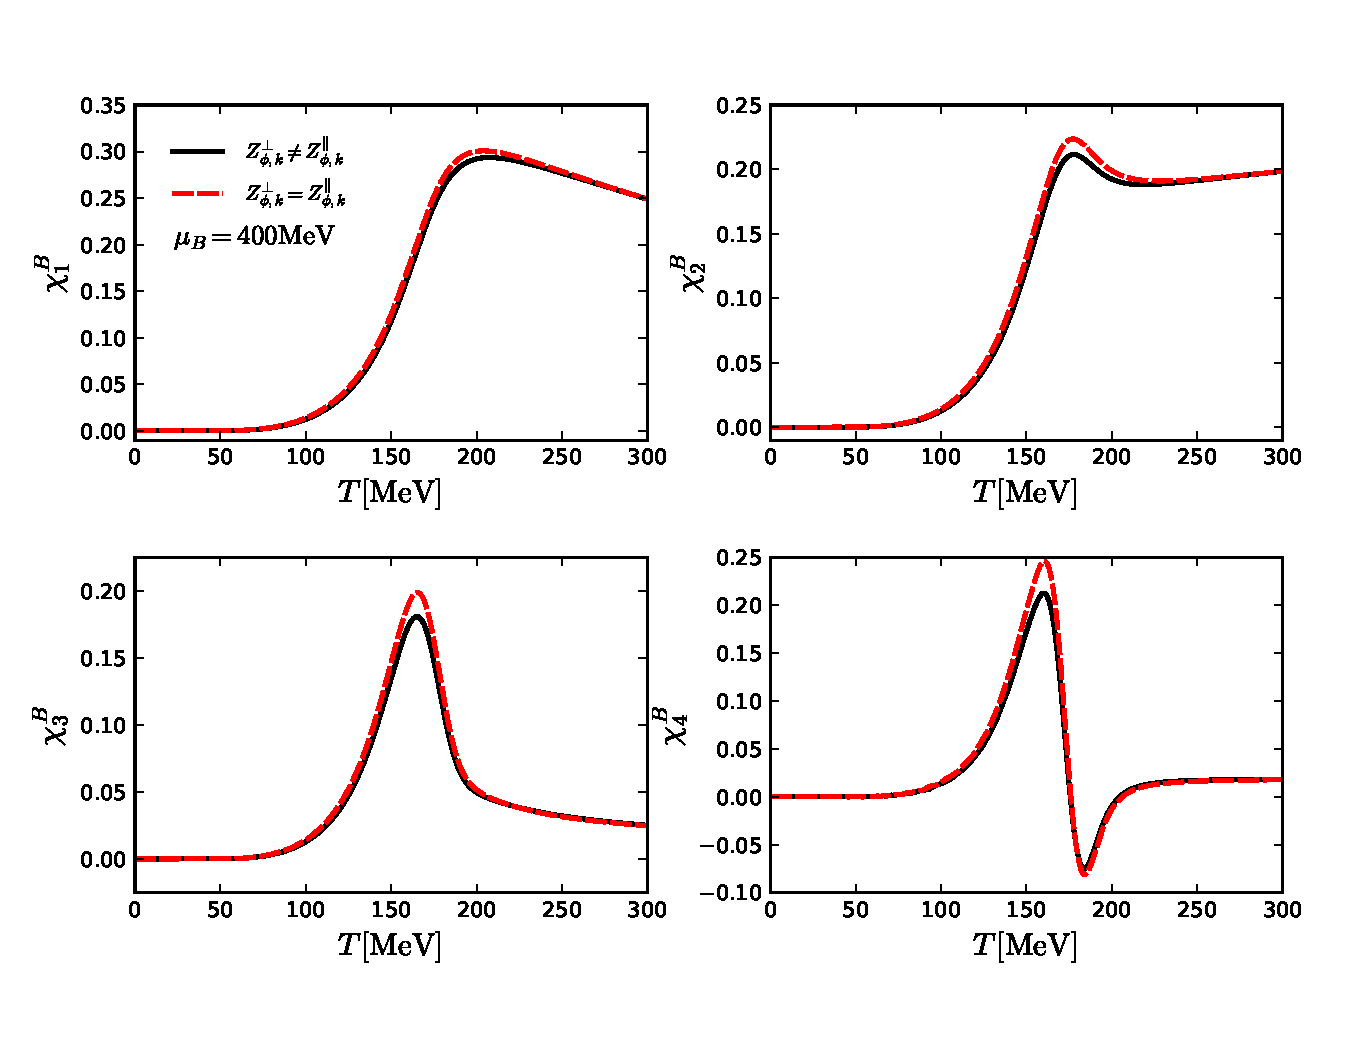
\includegraphics[width=1.0\textwidth]{4chi.pdf}
\caption{The first to the fourth order of the baryon number fluctuation, which are obtained under $Z^{\|}_{\phi}=Z^{\bot}_{\phi}$, $Z^{\|}_{\phi}\neq Z^{\bot}_{\phi}$ 
and fix point, physical point expansion of the effective potential. }
\end{figure*}

\begin{figure*}[t]
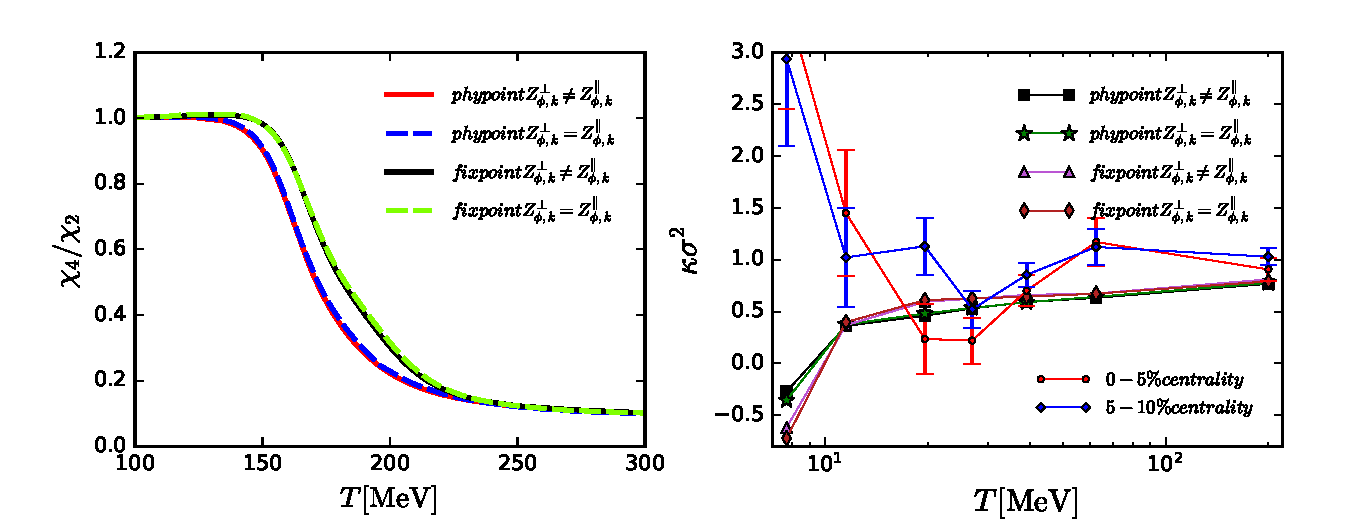
\includegraphics[width=1.0\textwidth]{kur.pdf}
\caption{The left curves are the kurtosis as the function of temperature. The right broken lines are the kurtosis as the function of collision energy.}
\label{fig:r42}
\end{figure*}

The fluctuation of the baryon number is related to some observables. The kurtosis of the baryon number fluctuation at different collision energy 
can be observed in the experiment like STAR. So the calculation of the baryon number fluctuation is important work. 
The definition of the each order baryon number fluctuation can be written as
\begin{align}\label{}
\begin{split}
\chi^{B}_{n}=\frac{\partial^n}{\partial(\mu_B/T)^n}\frac{p}{T^4}
\end{split}
\end{align} 
The baryon chemical potential satisfying the relationship of $\mu_B=3\mu$. The quadratic and quartic fluctuations can be expressed using the 
average baryon number fluctuation $\langle N_B \rangle$
\begin{align}\label{}
\begin{split}
\chi^{B}_{2}&=\frac{1}{VT^3}\langle \delta {N_B}^2 \rangle\\
\chi^{B}_{4}&=\frac{1}{VT^3}\left( \langle \delta {N_B}^4 \rangle-3\langle \delta {N_B}^2 \rangle^2 \right)
\end{split}
\end{align}

The definition of the kurtosis can be written as
\begin{align}
\kappa \sigma^2=\frac{\chi^{B}_{4}}{\chi^{B}_{2}}
\end{align}\par
At the same time, we calculated the chemical freeze-out line as the function of the collision energy and the kurtosis of the baryon
number fluctuation. The value of the kurtosis is determined by the temperature and the baryon chemical potential. We use the 
correspondence of the collision energy and chemical potential which is give in the Table~\ref{tab:cle}. We obtain the freeze-out 
temperature by the three and two order of the baryon number fluctuation $\chi^B_3/\chi^B_2$ under the different baryon chemical 
potential which are corresponding to the different collision energy. Then we can compare the numerical results between the fix point 
expansion and physical point expansion of the effective potential $V_k(\rho)$ and the results of splitted meson wave function 
renormalisation. There are many ways to determine the freeze-out temperature. 
\begin{table}[h]
  \centering
  \begin{tabular}[c]{c|clclclclclcl}
    \hline \hline
    $\sqrt{s}\,(\mathrm{GeV})$ & 200 & 62.4 & 39 & 27 & 19.6 & 11.5 & 7.7\\ \hline
    $\mu_{B,N_f=2}\,(\mathrm{MeV})$&25.3&78.1&121&168.7&222.7&343&459.4\\ \hline
  \end{tabular}
  \caption{The relationship of collision energy and baryon chemical potential }
  \label{tab:cle}
\end{table}

%%%%%%%%%%%%%%%%%%%%%%%%%%%%%%%%%%%
%%%%%%%%%%%%%%%%%%%%%%%%%%%%%%%%%%%%
\section{numerical results and conclusion}
In this work, we investigated the baryon number fluctuations and some thermodynamic quantities with in the functional 
renormalization group. We made a comparison of the results between the approximation of the mesonic wave function 
renormalizations and without the approximation. The calculation are accomplished under the fix point and physical point expansion of 
the effective potential.Now we give the initial conditions of our calculation. The initial UV scale is $\Lambda=700$MeV. At 
$k=\Lambda$ the initial effective potential can be written as

\begin{align}
V_\Lambda(\rho)=\frac{\lambda_\Lambda}{2}\rho^2+\nu_\Lambda\rho
\end{align}
And the parameter we chosen in the equation above is shown in the table below
\begin{table}[h]
\begin{tabular}{ccccc}
\hline
 &$\lambda_\Lambda$& $\nu_\Lambda$ & c & h \\
\hline
 $\kappa\,Z^{\|}_{\phi}=Z^{\bot}_{\phi}\,h_k$& 10.15 & 8.11$(GeV^2)$ & 0.2568$(GeV^3)$ & 7.274\\
 $\kappa\,Z^{\|}_{\phi}\neq Z^{\bot}_{\phi}\,h_k$& 10.15 & 8.17$(GeV^2)$ & 0.2568$(GeV^3)$ & 7.274\\
 $\kappa_k\,Z^{\|}_{\phi}=Z^{\bot}_{\phi}\,h_k$& 5.00 & 17.86$(GeV^2)$ & 0.3696$(GeV^3)$ & 10.110\\
 $\kappa_k\,Z^{\|}_{\phi}\neq Z^{\bot}_{\phi}\,h_k$& 11.00 & 17.91$(GeV^2)$ & 0.3684$(GeV^3)$ & 10.198\\
 
 
\hline
\end{tabular}
 \caption{The setting of the initial condition parameters.}
  \label{tab:para}
\end{table}
These four parameters are chosen by fitting the observables: $m_\pi=135.9$MeV, $m_\sigma=460.0$MeV, $f_\pi=92.1$MeV, $m_q=298.8$MeV.\par
In the end, we give the numerical calculation results of the physical quantity. In this section we will show the results of the comparison in the two flavor PQM model. 
Two comparisons have been made, one is $Z^{\|}_{\phi}=Z^{\bot}_{\phi}$ and $Z^{\|}_{\phi}\neq Z^{\bot}_{\phi}$, the other one is the fix point and physical 
point expansion of the effective potential. \par
As we can see in the \Fig{fig:m}, the pion mass and constituent quark mass as the function of temperature. It is clear that the pion mass under the physical point 
is larger at the high temperature, which means the pion is decoupling quicker. For the meson mass is related to the expansion of the effective potential, the expansion point is 
running with the cutoff scale k or not 
will of course influence the value of the pion mass. However, the split of the meson wave function renormalisation make little effect on the mass.\par
As is shown in the \Fig{fig:4chi}, because the baryon chemical potential has little influence to the numerical result of 
the $\chi^{B}_{2}$ and $\chi^{B}_{4}$, however the $\chi^{B}_{1}$ and $\chi^{B}_{3}$ are more sensitive to the chemical potential. Consequently, we give the 
odd order of the fluctuation under the chemical potential of 50 MeV and 100 MeV, and the even order under vanishing chemical potential. 
The results of the quartic fluctuations under two kinds of wave function renormalizations have larger difference at the peak of the curves, 
the results of $Z^{\bot}_{\phi,k}\neq Z^{\|}_{\phi,k} $ are little lower than the results of $Z^{\bot}_{\phi,k}= Z^{\|}_{\phi,k} $.\par
In the \Fig{fig:r42} we show $\kappa \sigma^2=\chi^{B}_{4}/\chi^{B}_{2}$ the kurtosis of the baryon number fluctuation. We can tell from the curves, the two kinds of 
$Z_\phi$ almost no effect on the kurtosis results. On the other hand, the influence of the running expansion point of the effective potential is greater. The physical point expansion 
suppress the kurtosis quicker as the temperature rises than the fix point expansion. It is expected from the results of the four order of the fluctuation.\par
In the \Fig{fig:fpitra} we give the pion decay constant and trace anomaly as a function of temperature. The left one is the pion decay constant. It is clear, the separation of 
the meson wave function renormalisation doesn't make much change. However, the running expansion point of the effective potential brings some differences at high 
temperature. The trace anomaly doesn't change much either under the different wave function renormalisation, and the physical point expansion suppress the value at high
temperature.



\begin{figure*}[t]
\label{fig:fpitra}
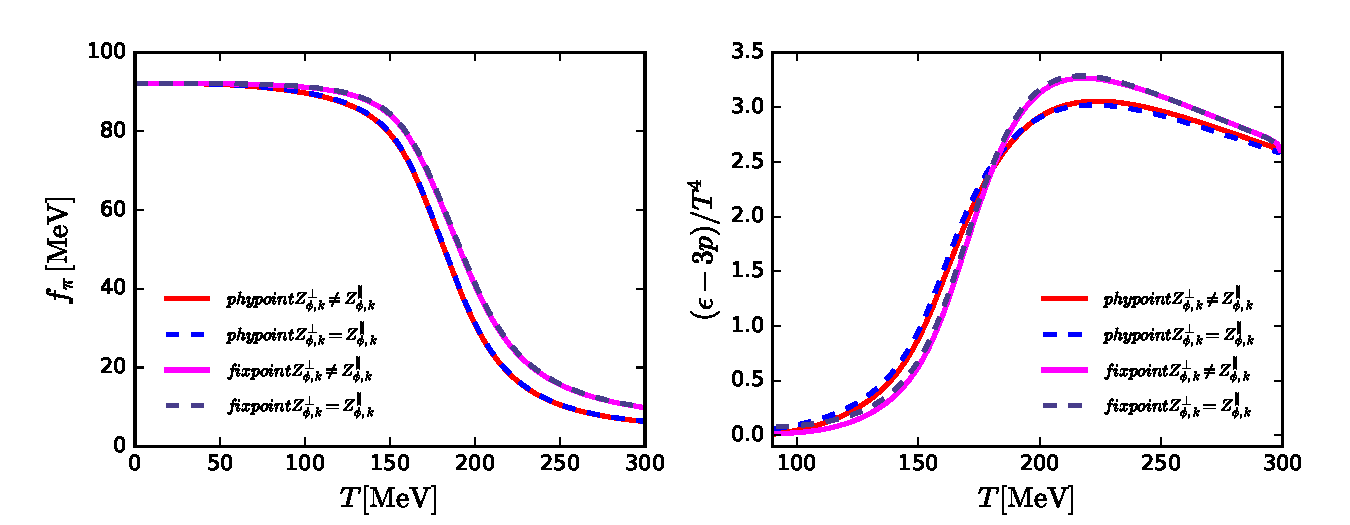
\includegraphics[width=1.0\textwidth]{fpitra.pdf}
\caption{}
\end{figure*}




%%%%%%%%%%%%%%%%%%%%%%%%%%%%%%%%%%%%
\acknowledgments
Thanks


%%%%%%%%%%%%%%%%%%%%%%%%%%%%%%%%%%%%%%%%%%%%%%%%%%%%%%%%%%%%%
%%%%%%%%%%%%%%%%%%%%%%%%%%%%%%%%%%%%%%%%%%%%%%%%%%%%%%%%%%%%%

\appendix

\section{Some useful formulas}
\label{app:formula}

In this work we use the $3d$- flat or Litim regulators \cite{Litim:2000ci,Litim:2001up}, which are very suited for the computations at finite temperature and densities, since the summation for the Matsubara frequencies is not affected by the $3d$ regulators, and can be performed analytically. The regulators in \Eq{eq:WetterichEqPQM} read
\begin{align}
  R^{\phi}_{k}(q_0,\bm{q})&=Z^{\perp}_{\phi,k}\bm{q}^2 r_B(\bm{q}^2/k^2)\,, \label{eq:Rphi}\\[2ex] 
  R^{q}_{k}(q_0,\bm{q})&=Z_{q,k}i\bm{\gamma} \cdot \bm{q} r_F(\bm{q}^2/k^2)\,, \label{eq:Rq}
\end{align} 
with 
\begin{align}
  r_B(x)&=\left( \frac{1}{x}-1 \right)\Theta(1-x)\,,\\[2ex] 
  r_F(x)&=\left( \frac{1}{\sqrt{x}}-1 \right)\Theta(1-x)\,,  \label{}
\end{align} 
where $\Theta(x)$ is the Heaviside step function. Note that since $Z^{\perp}_{\phi,k}\neq Z^{\parallel}_{\phi,k}$, it is  the transversal wave function renormalization for the meson appearing in \Eq{eq:Rphi}.


















in which
Then we give a definition to the meson and quark propagator
\begin{align}
\begin{split}
G_\phi(q,\bar{m}^{2}_{\phi,k})&=\frac{1}{z_\phi\tilde{q}^{2}_{0}+1+\bar{m}^{2}_{\phi,k}} ,\\
G_q(q,\bar{m}^{2}_{q,k})&=\frac{1}{z^{2}_{q}(\tilde{q}_0+i\tilde{\mu})^2+1+\bar{m}^{2}_{q,k}}
\end{split}
\end{align} 
in the equation above we have $\tilde{q}_0=q_0/k$, $\tilde{\mu}=\mu/k$ and for the fermions we have
$q_0=(2n_q+1)\pi T \ (n_q\in \mathbb{Z})$ for the bosons we have $q_0=2n_q\pi T$. Here $z=Z^\|/Z^\bot$ is the ratio of the 
two components of the wave function renormalizations. In this work we choose $z_q=1$ which means $Z^{\|}_{q}=
Z^{\bot}_{q}$ and $z_\phi\neq 1$ which means $Z^{\|}_{\phi}\neq Z^{\bot}_{\phi}$. To obtain the threshold functions, we 
define


in the equations above the form of the distribution functions are
\begin{align}
\begin{split}
n_B(\bar{m}^{2}_{\phi,k},z_\phi;T)=\frac{1}{\exp\lbrace \frac{1}{T}\frac{k}{z_\phi^{1/2}}\sqrt{1+\bar{m}^{2}_{\phi,k}}
\rbrace-1}
\end{split}
\end{align} 
and
\begin{align}
\begin{split}
n_F(\bar{m}^{2}_{q,k},z_\phi;T)=\frac{1}{\exp\lbrace \frac{1}{T}\frac{k}{z_q}\sqrt{1+\bar{m}^{2}_{q,k}}-\mu 
\rbrace+1}
\end{split}
\end{align} 
In the effective potential's flow equation, there are bosonic and fermionic threshold functions. The anomalous dimension 
of the mesonic field has change into the transverse component of it. The form of the threshold functions are
\begin{align}
\begin{split}
l_0^{(B,d)}(\bar{m}^{2}_{\phi,k},\eta^\bot_{\phi,k};T)=\frac{2}{d-1}\left( 1- \frac{\eta^{\bot}_{\phi,k}}{d+1}\right) 
\mathcal{B}_{(1)}(\bar{m}^{2}_{\phi,k},z_\phi;T)
\end{split}
\end{align} 
and
\begin{align}
\begin{split}
l_0^{(F,d)}&(\bar{m}^{2}_{q,k},\eta_{q,k};T,\mu)\\&=\frac{2}{d-1}\left( 1-\frac{\eta_{q,k}}{d} \right)\mathcal{F}_{(1)}
(\bar{m}^{2}_{q,k},z_q=1;T,\mu)
\end{split}
\end{align} 
The definition of the threshold function $\mathcal{BB}_{(1,1)}$ is
\begin{align}
\begin{split}
\mathcal{BB}_{(1,1)}&(\bar{m}^{2}_{\phi_a,k},\bar{m}^{2}_{\phi_b,k},z_\phi;T)\\
&=-\frac{T}{k}\sum_{n_q}G_\phi(q,\bar{m}^{2}_{\phi_a,k})G_\phi(q,\bar{m}^{2}_{\phi_b,k})
\end{split}
\end{align} 
then we can obtain the $\mathcal{BB}_{(2,2)}$ in a same way
\begin{align}
\begin{split}
\mathcal{BB}_{(2,2)}&(\bar{m}^{2}_{\phi_a,k},\bar{m}^{2}_{\phi_b,k},z_\phi;T)\\
&=\frac{\partial^2}{\partial\bar{m}^{2}_{\phi_a,k}\partial\bar{m}^{2}_{\phi_b,k}}\mathcal{BB}_{(1,1)}(\bar{m}^{2}_{\phi_a,k}
\bar{m}^{2}_{\phi_b,k},z_\phi;T)
\end{split}
\end{align} 
The expression of the $\mathcal{BB}_{(1,1)}$ is 
%\begin{widetext}
\begin{align}
\begin{split}
&\mathcal{BB}_{(1,1)}(\bar{m}^{2}_{\phi_a,k},\bar{m}^{2}_{\phi_b,k},z_\phi;T)=\\&-\frac{1}{z^{1/2}_{\phi}}\left\{ \left( 
\frac{1}{2}+n_B(\bar{m}^{2}_{\phi_a,k},z_\phi;T) \right)\frac{1}{(1+\bar{m}^{2}_{\phi_a,k})^{1/2}} \right. \\
&\left.\times \frac{1}{\bar{m}^{2}_{\phi_a,k}-\bar{m}^{2}_{\phi_b,k}}+\left( \frac{1}{2}+n_B(\bar{m}^{2}_{\phi_b,k},z_\phi;T) 
\right)\right. \\
&\left.\times \frac{1}{(1+\bar{m}^{2}_{\phi_b,k})^{1/2}}\frac{1}{\bar{m}^{2}_{\phi_b,k}-\bar{m}^{2}_{\phi_a,k}}\right\}
\end{split}
\end{align} 
%\end{widetext}
then we can get the expression of the threshold functions of any $n$.
The definition of the $L^{(4)}_{(1,1)}$ in the flow equation of the Yukawa coupling is
\begin{align}
\begin{split}
L^{(4)}_{(1,1)}&(\bar{m}^{2}_{q,k},\bar{m}^{2}_{\phi,k},\eta_{q,k},\eta_{\phi,k};T,\mu)\\
&=\frac{2}{3}\bigg[(1-\frac{\eta_{\phi,k}}{5})\mathcal{FB}_{(1,2)}(\bar{m}^{2}_{q,k},\bar{m}^{2}_{\phi,k};T,\mu)\\
&+(1-\frac{\eta_{q,k}}{4})\mathcal{FB}_{(2,1)}(\bar{m}^{2}_{q,k},\bar{m}^{2}_{\phi,k};T,\mu)\bigg]
\end{split}
\end{align} 
The higher order of the function $L$ can be obtain by the derivation of the square of mass. The expression of the threshold function $\mathcal{FB}$  
is
\begin{align}
\begin{split}
\mathcal{FB}_{(1,1)}&(\bar{m}^{2}_{q,k},\bar{m}^{2}_{\phi,k};T,\mu,p_0)\\
&=\frac{T}{k}\sum_{n_q}G_{\phi}(p-q,\bar{m}^{2}_{\phi,k})G_q(q,\bar{m}^{2}_{q,k})
\end{split}
\end{align} 

%%%%%%%%%%%%%%%%%%%%%%%%%%%%%%%%%%%%%%%%%%%%%


\section{}
In order to obtain the flow equation of the effective potential, the mesonic anomalous dimensions are needed. Because 
we have divided the wave function renormalizations into the transversal and longitudinal components, so the 
anomalous dimensions should be divided either.
The analytical form of the mesonic anomalous dimensions can be written like
\begin{align}
\begin{split}
\eta_{\phi,k}^{\|}
&=\frac{1}{6\pi^2}\bigg\{ 
 \frac{4}{k^2z_\phi^4}\bar{\kappa}_k(\bar{V}''_k(\bar{\kappa}_k))^2\bigg[ 
 -6\mathcal{BB}_{(2,2)}(\bar{m}^{2}_{\pi,k},\bar{m}^{2}_{\sigma,k};T)\\
&+\frac{4}{z_\phi}(1+\bar{m}^{2}_{\sigma}){\mathcal{BB}}_{(2,3)}(\bar{m}^{2}_{\pi,k},\bar{m}^{2}_{\sigma,k};T)\\
&+\frac{4}{z_\phi}(1+\bar{m}^{2}_{\pi}){\mathcal{BB}}_{(3,2)}(\bar{m}^{2}_{\pi,k},\bar{m}^{2}_{\sigma,k};T)\bigg]\\
&\times(1-\frac{1}{5}\eta^{\bot}_{\phi,k})+\frac{N_c\bar{h}^{2}_{k}}{z_\phi}\mathcal{F}_{(3)}(\bar{m}^{2}_{q,k};T,\mu)(4-\eta_{q,k})\bigg\}   
\end{split}
\end{align} 
and the other component
\begin{align}
\begin{split}
\eta_{\phi,k}^{\bot}
&=\frac{1}{6\pi^2}\bigg\{ 
\frac{4}{k^2z_\phi^4}\bar{\kappa}_k(\bar{V}''_k(\bar{\kappa}_k))^2 \mathcal{BB}_{(2,2)}(\bar{m}^{2}_{\pi,k},\bar{m}^{2}_{\sigma,k};T)
\\&+N_c\bar{h}^{2}_{k}\bigg[\mathcal{F}_{(2)}(\bar{m}^{2}_{q,k};T,\mu)(2\eta_{q,k}-3)\\
&-4(\eta_{q,k}-2)\mathcal{F}_{(3)}(\bar{m}^2_{q,k};T,\mu)\bigg]
\bigg\}   
\end{split}
\end{align} 


%%%%%%%%%%%%%%%%%%%%%%%%%%%%%%%%%%%%%%%%%%%%

Now we can obtain the form of the quark anomalous dimension
\begin{align}
\begin{split}
\eta_{q,k}=&\frac{1}{24\pi^2N_f}(4-\eta_{\phi,k})\bar{h}^{2}_{k}\\
&\times\bigg\{ (N^{2}_{f}-1)\mathcal{FB}_{(1,2)}(\bar{m}^{2}_{q,k},\bar{m}^{2}_{\pi,k};T,\mu,p_{0,ex})\\
&+\mathcal{FB}_{(1,2)}(\bar{m}^{2}_{q,k},\bar{m}^{2}_{\sigma,k};T,\mu,p_{0,ex}) \bigg\}
\end{split}
\end{align} 

%%%%%%%%%%%%%%%%%%%%%%%%%%%%%%%%%%%%%%%%%%%%

% The \nocite command causes all entries in a bibliography to be
% printed out whether or not they are actually referenced in the
% text. This is appropriate for the sample file to show the different
% styles of references, but authors most likely will not want to use
% it.  \nocite{*}

%\bibliography{refspec}% Produces the bibliography via BibTeX.
\bibliography{ref-lib}% Produces the bibliography via BibTeX.


\end{document}